\documentclass[11pt]{article}
\usepackage[pdftex]{graphicx, color}
\usepackage{amsmath}
\usepackage{listings}
\usepackage{ebproof}

\usepackage{tikz}
\usetikzlibrary{automata,positioning}

\headheight 8pt \headsep 20pt \footskip 30pt
\textheight 9in \textwidth 6.5in
\oddsidemargin 0in \evensidemargin 0in
\topmargin -.35in

\lstset{basicstyle=\small\ttfamily,breaklines=true,numbers=left}

\usepackage{array}
\newcolumntype{L}[1]{>{\raggedright\let\newline\\\arraybackslash\hspace{0pt}}m{#1}}
\newcolumntype{C}[1]{>{\centering\let\newline\\\arraybackslash\hspace{0pt}}m{#1}}
\newcolumntype{R}[1]{>{\raggedleft\let\newline\\\arraybackslash\hspace{0pt}}m{#1}}

\begin{document}
\begin{center}
%% Change this:
\LARGE Nan Bai - nancybai\\
\Large CS143 - Written Assignment 4
\end{center}

% A pdf file can be generated from this by running
% pdflatex -jobname=WA4_solved WA4_template.tex
% Upload WA4_solved.pdf to GradeScope
% to submit the assignment!

This assignment covers code generation, operational semantics and optimization. You may discuss this assignment with other students and work on the problems together. However, your write-up should be your own individual work, and you should indicate in your submission who you worked with, if applicable. Assignments can be submitted electronically through Gradescope as a PDF by Tuesday, June 6, 2017 11:59 PM PDT. A \LaTeX \ template for writing your solutions is available on the course website.

\begin{enumerate}
  % Problem 1
  \item \textbf{(20 pts)} Consider the following program in Cool, representing an over-engineered implementation which calculates the factorial of 3 using an operator class and a reduce() method:
  \begin{lstlisting}
    class BinOp {
        operate(a: Int, b: Int): Int {
            a + b
        };
        optype(): String {
            "BinOp"
        };
    };
    class SumOp inherits BinOp { 
        optype(): String {
            "SumOp"
        };
    };
    class MulOp inherits BinOp {
        operate(a: Int, b: Int): Int {
            a * b
        };
        optype(): String {
            "MulOp"
        };
    };
    class IntList {
        head: Int;
        tail: IntList;
        empty_tail: IntList; -- Do not assign.
        tail_is_empty(): Bool {
            tail = empty_tail
        };
        get_head(): Int { head };
        set_head(n: Int): Int {
            head <- n
        };
        get_tail(): IntList { tail };
        set_tail(t: IntList): IntList {
            tail <- t
        };
        generate(n: Int): IntList {
            let l: IntList <- New IntList in {
                -- Point A
                l.set_head(n);
                if (n = 1) then
                    l.set_tail(empty_tail)
                else
                    l.set_tail(generate(n-1))
                fi;
                l;
            }
        };
    };
    class Main {
        reduce(result: Int, op: BinOp, l: IntList): Int {{
            result <- op.operate(result,l.get_head());
            if (l.tail_is_empty() = true) then
                -- Point B
                result
            else
                reduce(result,op,l.get_tail())
            fi;
        }};
        main(): Object {
            let op: BinOp <- New MulOp, l: IntList <- New IntList, io: IO <- New IO in {
                l <- l.generate(3); 
                io.out_int(self.reduce(1,op,l));
            }
        };
    };
  \end{lstlisting}
  
  The following is an abstracted representation of a memory layout of the program generated by a hypothetical Cool compiler for the above code (note that this might or might not correspond to the layout generated by your compiler or the reference coolc):
  
  \begin{tabular}{ | c | }
  \hline
  \textbf{Code segment:} \\
  \begin{tabular}{ | R{2cm} | L{9cm} |}
  \hline
  $\mathtt{maddr}_1$: & \texttt{cgen\_m(BinOp.operate)} \\
  \cline{2-2}
  $\mathtt{maddr}_2$: & \texttt{cgen\_m(BinOp.optype)} \\
  \cline{2-2}
  $\mathtt{maddr}_3$: & \texttt{cgen\_m(SumOp.optype)} \\
  \cline{2-2}
  $\mathtt{maddr}_4$: & \texttt{cgen\_m(MulOp.operate)} \\
  \cline{2-2}
  $\mathtt{maddr}_5$: & \texttt{cgen\_m(MulOp.optype)} \\
  \cline{2-2}
  $\mathtt{maddr}_6$: & \texttt{cgen\_m(IntList.tail\_is\_empty)} \\
  \cline{2-2}
  $\mathtt{maddr}_7$: & \texttt{cgen\_m(IntList.get\_head)} \\
  \cline{2-2}
  $\mathtt{maddr}_8$: & \texttt{cgen\_m(IntList.set\_head)} \\
  \cline{2-2}
  $\mathtt{maddr}_9$: & \texttt{cgen\_m(IntList.get\_tail)} \\
  \cline{2-2}
  $\mathtt{maddr}_{10}$: & \texttt{cgen\_m(IntList.set\_tail)} \\
  \cline{2-2}
  $\mathtt{maddr}_{11}$: & \texttt{cgen\_m(IntList.generate)} \\
  \cline{2-2}
  $\mathtt{maddr}_{12}$: & \texttt{cgen\_m(Main.reduce)} \\
  \cline{2-2}
  $\mathtt{maddr}_{13}$: & \texttt{cgen\_m(Main.main)} \\
  \hline
  \end{tabular} \\
  \textbf{Dispatch tables:} \\
  \begin{tabular}{ | R{2cm} | L{9cm} |}
  \hline
  $\mathtt{maddr}_{14}$: & \texttt{DT[BinOp]} \\
  \cline{2-2}
  $\mathtt{maddr}_{15}$: & \texttt{DT[SumOp]} \\
  \cline{2-2}
  $\mathtt{maddr}_{16}$: & \texttt{DT[MulOp]} \\
  \cline{2-2}
  $\mathtt{maddr}_{17}$: & \texttt{DT[IntList]} \\
  \cline{2-2}
  $\mathtt{maddr}_{18}$: & \texttt{DT[Main]} \\
  \hline
  \end{tabular} \\
  \textbf{Stack} ($\mathtt{maddr}_{19}$) \\
  $\downarrow$ \\
  \\
  \\
  \\
  \hline
  \\
  \\
  \\
  $\uparrow$ \\
  \textbf{Heap} \\
  \hline
  \end{tabular}
  
  In the above, $\mathtt{maddr}_i$ represents the memory address at which the corresponding method's code or dispatch table starts. You should assume that the above layout is contiguous in memory.
  
  \begin{enumerate}
    \item \textbf{(4 pts)} Assume the MIPS assembly code to be stored starting at address $\mathtt{maddr}_{12}$ and ending immediately before $\mathtt{maddr}_{13}$ (i.e. not including the instruction starting at $\mathtt{maddr}_{13}$) was generated using the code generation process from lecture. In particular, assume that the caller is responsible for saving and restoring the frame pointer. In addition, assume that the address to the self object is stored on the stack along with the other parameters. How many instructions using the frame pointer register ($\$fp$) will be present within such code? Why?\\
    \textbf{Answer:} \\
    10 instructions with $\$fp$ will be present with such code. The Main.reduce method called 5 methods (BinOp.operate(), IntList.get\_head(), IntList.tail\_is\_emtpy(), Main.reduce() and IntList.get\_tail()) within its body and each time caller needs to save and restore their frame pointers.
    
   \newpage
    \item \textbf{(4 pts)} The following is a representation of the dispatch table for class Main: \\
    
    \begin{tabular}{ | l | l | l | }
    \hline
    Method Idx & Method Name & Address \\
    \hline
    0 & reduce & $\mathtt{maddr}_{12}$ \\
    \hline
    1 & main & $\mathtt{maddr}_{13}$ \\
    \hline
    \end{tabular} \\
    
    Provide equivalent representations for the dispatch tables of BinOp, SumOp, MulOp, and IntList.\\
    \textbf{Answer:} \\
	dispatch table for class BinOp: \\
    \begin{tabular}{ | l | l | l | }
    \hline
    Method Idx & Method Name & Address \\
    \hline
    0 & operate & $\mathtt{maddr}_{1}$ \\
    \hline
    1 & optype & $\mathtt{maddr}_{2}$ \\
    \hline
    \end{tabular} \\
	
	dispatch table for class SumOp: \\
	\begin{tabular}{ | l | l | l | }
    \hline
    Method Idx & Method Name & Address \\
    \hline
    0 & operate & $\mathtt{maddr}_{1}$ \\
    \hline
    1 & optype & $\mathtt{maddr}_{3}$ \\
    \hline
    \end{tabular} \\
	
	dispatch table for class MulOp: \\
	\begin{tabular}{ | l | l | l | }
    \hline
    Method Idx & Method Name & Address \\
    \hline
    0 & operate & $\mathtt{maddr}_{4}$ \\
    \hline
    1 & optype & $\mathtt{maddr}_{5}$ \\
    \hline
    \end{tabular} \\
	
	dispatch table for class IntList: \\
	\begin{tabular}{ | l | l | l | }
    \hline
    Method Idx & Method Name & Address \\
    \hline
    0 & tail\_is\_emtpy & $\mathtt{maddr}_{6}$ \\
    \hline
    1 & get\_head & $\mathtt{maddr}_{7}$ \\
	\hline
    1 & set\_head & $\mathtt{maddr}_{8}$ \\
	\hline
    1 & get\_tail & $\mathtt{maddr}_{9}$ \\
	\hline
    1 & set\_tail & $\mathtt{maddr}_{10}$ \\
	\hline
    1 & generate & $\mathtt{maddr}_{11}$ \\
	\hline
    \end{tabular} \\
    
   \newpage
    \item \textbf{(4 pts)} Consider the state of the program at runtime when reaching (for the first time) the beginning of the line marked with the comment ``Point A''. Give the object layout (as per Lecture 12) of every object currently on the heap which is of a class defined by the program (i.e. ignoring Cool base classes such as IO or Int). For attributes, you can directly represent Int values by integers and an unassigned pointer by \textbf{void}. However, note that in a real Cool program, Int is an object and would have its own object layout, omitted here for simplicity. Finally, you can assume class tags are numbers from 1 to 5 given in the same order as the one in which classes appear in the layout above, and that attributes are laid out in the same order as the class definition.\\
    \textbf{Answer:} \\
	
    \begin{tabular}{|c|c|c|c|c|c|c|}
    \hline
    Offset Class & 0 & 4 & 8 & 12 & 16 & 20 \\
    \hline
    op & 1 & 3 & $\mathtt{maddr}_{16}$ &  &  &  \\
    \hline
    l & 2 & 6 & $\mathtt{maddr}_{17}$ & 0 & void & void \\
    \hline
    l & 3 & 6 & $\mathtt{maddr}_{17}$ & 0 & void & void \\
    \hline
    \end{tabular} \\
	
    
   \newpage

    \item \textbf{(8 pts)} The following table represents an abstract view of the layout of the stack at runtime when reaching (for the first time) the beginning of the line marked with the comment ``Point A''. \\
    
    \begin{tabular}{ | r | l | c | l | }
    \hline
    Address & Method & Contents & Description \\
    \hline
    $\mathtt{maddr}_{19}$ & Main.main & self & $\mbox{arg}_0$ \\
    \hline
    $\mathtt{maddr}_{19}+4$ & Main.main & ... & Return \\
    \hline
    $\mathtt{maddr}_{19}+8$ & Main.main & op & local \\
    \hline
    $\mathtt{maddr}_{19}+12$ & Main.main & l & local \\
    \hline
    $\mathtt{maddr}_{19}+16$ & Main.main & io & local \\
    \hline
    $\mathtt{maddr}_{19}+20$ & IntList.generate & $\mathtt{maddr}_{19}$ & FP \\
    \hline
    $\mathtt{maddr}_{19}+24$ & IntList.generate & self & $\mbox{arg}_0$ \\
    \hline
    $\mathtt{maddr}_{19}+28$ & IntList.generate & 3 & $\mbox{arg}_1$ \\
    \hline
    $\mathtt{maddr}_{19}+32$ & IntList.generate & $\mathtt{maddr}_{13}+\delta$ & Return \\
    \hline
    $\mathtt{maddr}_{19}+36$ & IntList.generate & l & local \\
    \hline
    \end{tabular} \\
    
    Give a similar view of the stack at runtime when reaching (for the first time) the beginning of the line marked with the comment ``Point B''.\\

    Note that we are assuming there are no stack frames above Main.main(...). This doesn't necessarily match a real implementation of the Cool runtime system, where main must return control to the OS or the Cool runtime on exit. For the purposes of this exercise, feel free to ignore this issue. Also, since you don't have the generated code for every method above, you cannot directly calculate the return address to be stored on the stack. You should however give it as $\mathtt{maddr}_{i}+\delta$, denoting an unknown address between $\mathtt{maddr}_{i}$ and $\mathtt{maddr}_{i+1}$. This notation is used in the example above. For locals, you should use the variable name, but remember that in practice it is the heap address that gets stored in memory for objects.\\
    \textbf{Answer:} \\
    \begin{tabular}{ | r | l | c | l | }
    \hline
    Address & Method & Contents & Description \\
    \hline
    $\mathtt{maddr}_{19}$ & Main.main & self & $\mbox{arg}_0$ \\
    \hline
    $\mathtt{maddr}_{19}+4$ & Main.main & ... & Return \\
    \hline
    $\mathtt{maddr}_{19}+8$ & Main.main & op & local \\
    \hline
    $\mathtt{maddr}_{19}+12$ & Main.main & l & local \\
    \hline
    $\mathtt{maddr}_{19}+16$ & Main.main & io & local \\
    \hline
    $\mathtt{maddr}_{19}+20$ & IO.out_int & $\mathtt{maddr}_{19}$ & FP \\
    \hline
    $\mathtt{maddr}_{19}+24$ & IO.out_int & self & $\mbox{arg}_0$ \\
	\hline
    $\mathtt{maddr}_{19}+28$ & IO.out_int & $\mathtt{maddr}_{13}+\delta$ & Return \\
    \hline
    $\mathtt{maddr}_{19}+32$ & Main.reduce & $\mathtt{maddr}_{19}+24$ & FP \\
    \hline
    $\mathtt{maddr}_{19}+36$ & Main.reduce & self & $\mbox{arg}_0$ \\
    \hline
    $\mathtt{maddr}_{19}+40$ & Main.reduce & 1 & $\mbox{arg}_1$ \\	
	\hline
    $\mathtt{maddr}_{19}+44$ & Main.reduce & op & $\mbox{arg}_2$ \\
	\hline
    $\mathtt{maddr}_{19}+48$ & Main.reduce & l & $\mbox{arg}_3$ \\
	\hline
    $\mathtt{maddr}_{19}+52$ & Main.reduce & $\mathtt{maddr}_{13}+\delta$ & Return \\
	\hline
    $\mathtt{maddr}_{19}+56$ & Main.reduce & result & local \\
    \hline
    \end{tabular} \\
    
   \newpage
    
  \end{enumerate}
  
  % Problem 2 
  \item \textbf{(4 pts)} Consider the following arithmetic expression: $7*((6+4)/2 - 3 + (5-4)*3) + 1$.
  
  \begin{enumerate}
    \item \textbf{(2 pts)} You are given MIPS code that evaluates this expression using a stack machine with a single accumulator register (similar to the method given in class Lecture 12). This code is wholly unoptimized and does not perform transformations such as arithmetic simplification or constant folding. How many times in total will this code push a value to or pop a value from the stack (give a separate count for the number of pushes and the number of pops)?\\
    \textbf{Answer:} 
    8 pushes and 8 pops
    
    \item \textbf{(2 pts)} Now suppose that you have access to two registers r1, r2 in addition to the stack pointer. Consider the code generated using the revised process described in lecture 12 starting on slide 30, with r1 as an accumulator and r2 storing temporaries. How many loads and stores are now required?\\
    \textbf{Answer:} 
    1 load and 1 store
  \end{enumerate}
  \newpage
    
  % Problem 3 
  \item \textbf{(16 pts)} Suppose you want to add a for-loop construct to Cool, having the following syntax:\\
  
  $$\mbox{for}\ \mbox{id}: \mbox{Int}\ \leftarrow e_1\ \mbox{to}\ e_2\ \mbox{do}\ e_3\ \mbox{rof}$$ 
  
  The above for-loop expression is evaluated as follows: expressions $e_1$ and $e_2$ are evaluated \underline{\emph{only once}}, then the body of the loop ($e_3$) is executed once for every integer in the range $[e_1, e_2]$ (inclusive) in order. Similar to the while loop, the for-loop returns void. Also assume that $id$ is not in the environment and hence cannot be modified in the loop body.
  
   \begin{enumerate}
    \item \textbf{(10 pts)} Give the operational semantics for the for-loop construct above.\\
    \textbf{Answer:} 
    
    \begin{prooftree}
    let $t_1$ and $t_2$ to be the temporary variable storing the value of $e_1$ and $e_2$, we have the following operational semantics where $S_3$ is the initial state before entering the for-loop. \\
    if $id$ is outside the range of $[e_1,e_3]$, the rule will be like
    \hypo[]{\mbox{so, E, S} \vdash e_1: v_1, S_1}
    \infer[no rule]1{\mbox{so, E, S_1} \vdash e_2: v_2, S_2}
    \infer[no rule]1{l_i = $newloc$(S_2)\  $for$\  i = 1, 2, 3}
    \infer[no rule]1{E' = E[t_1/l_1,t_2/l_2, id/l_3]}
    \infer[no rule]1{S_4 = S_2[v_1/l_1,v2/l_2, v_1/id]}
    \infer[no rule]1{\mbox{so, E', S_4} \vdash id >= t1\ and\ id <= t2: Bool(false), S_4}
    \infer2[]{\mbox{so, E, S} \vdash $for$\ id\leftarrow e_1\ \mbox{to}\ e_2\ \mbox{do}\ e_3\ \mbox{rof}: void, S_4}
    \end{prooftree}
    
    \newline
    if  $id$ is within the range, the rule will be like
    
    \begin{prooftree}
    \hypo[]{\mbox{so, E, S} \vdash e_1: v_1, S_1}
    \infer[no rule]1{\mbox{so, E, S_1} \vdash e_2: v_2, S_2}
     \infer[no rule]1{\mbox{so, E, S_2} \vdash e_3: v, S_3}
    \infer[no rule]1{l_i = $newloc$(S_3)\  $for$\  i = 1, 2, 3}
    \infer[no rule]1{E' = E[t_1/l_1,t_2/l_2, id/l_3]}
    \infer[no rule]1{S_4 = S_3[v_1/l_1,v2/l_2, v_1/id]}
    \infer[no rule]1{\mbox{so, E', S_4} \vdash id >= t1\ and\ id <= t2: Bool(true), S_4}
    \infer[no rule]1{\mbox{so, E', S_4} \vdash $for$\ id\leftarrow e_1\ \mbox{to}\ e_2\ \mbox{do}\ e_3\ \mbox{rof}: void, S_4}
    \infer2[]{\mbox{so, E, S} \vdash $for$\ id\leftarrow e_1\ \mbox{to}\ e_2\ \mbox{do}\ e_3\ \mbox{rof}: void, S_4}
    \end{prooftree}
    \newpage
    
    \item \textbf{(6 pts)} Give the code generation function $\mbox{cgen}(\mbox{for}\ \mbox{id}: \mbox{Int}\ \leftarrow e_1\ \mbox{to}\ e_2\ \mbox{do}\ e_3\ \mbox{rof})$ for this construct. Use the code generation conventions from the lecture. The result of $\mbox{cgen}(...)$ must be MIPS code following the stack-machine with one accumulator model.\\
    \textbf{Answer:} \\
    cgen(for id $\leftarrow$ $e_1$ to $e_2$ do $e_3$ rof): \newline \\
    cgen($e_1$) \\
    sw \$a0 0(\$sp) \# use this address to store $id$ \\
    sw \$a0 -4(\$sp) \# this address to store $e_1$ \\
    addiu \$sp \$sp -8 \\
    cgen($e_2$) \\
    sw \$a0 0(\$sp) \\
    addiu \$sp \$sp -4 \\
    \# enter the loop \\
    begin\_loop: \\
    lw \$t1 12(\$sp) \# $id$ \\
    lw \$t2 4(\$sp) \# $e_2$ \\
    lw \$t3 8(\$sp) \# $e_1$ \\
    blt \$t1 \$t3 end\_loop \\
    bgt \$t1 \$t2 end\_loop \\
    addi \$t1 \$t1 1 \\
    cgen($e_3$) \\
    b begin\_loop \\
    end\_loop: \\
    li \$a0 0
    
   \newpage
  \end{enumerate}
  
  % Problem 4
  \item \textbf{(8 pts)} Consider the following basic block, in which all variables are integers.
  
  \begin{lstlisting}
    a := f * f
    b := 1 * f + 0
    c := 7 * 7
    d := b + c
    e := f * f
    g := a + d
    x := e + d
    k := b * f
    h := g * x
    y := h + k
  \end{lstlisting}
  
  Assume that the only variables that are live at the exit of this block are x and y, while f is given as an input. In order, apply the following optimizations to this basic block. Show the result of each transformation. For each optimization, you must continue to apply it until no further applications of that transformation are possible, before writing out the result and moving on to the next.
  
  \begin{enumerate}
    \item Algebraic simplification
	
    \item Copy propagation
    \item Common sub-expression elimination
    \item Constant folding
    \item Copy propagation
    \item Dead code elimination
  \end{enumerate}

  
  When you have completed the last of the above transformations, the resulting program will still not be optimal. What optimization(s), in what order, can you apply to optimize the result further?\\
    \textbf{Answer:} 
 
    \begin{enumerate}
    \item Algebraic simplification
	  \begin{lstlisting}
    a := f * f
    b := f
    c := 7 * 7
    d := b + c
    e := f * f
    g := a + d
    x := e + d
    k := b * f
    h := g * x
    y := h + k
  \end{lstlisting}
  
    \item Copy propagation
	\begin{lstlisting}
    a := f * f
    b := f
    c := 7 * 7
    d := f + c
    e := f * f
    g := a + d
    x := e + d
    k := f * f
    h := g * x
    y := h + k
  \end{lstlisting}
  
    \item Common sub-expression elimination
	\begin{lstlisting}
    a := f * f
    b := f
    c := 7 * 7
    d := f + c
    e := a
    g := a + d
    x := e + d
    k := a
    h := g * x
    y := h + k
  \end{lstlisting}
  
  
    \item Constant folding
	\begin{lstlisting}
    a := f * f
    b := f
    c := 14
    d := f + c
    e := a
    g := a + d
    x := e + d
    k := a
    h := g * x
    y := h + k
  \end{lstlisting}
	
  
    \item Copy propagation
	
	\begin{lstlisting}
    a := f * f
    b := f
    c := 14
    d := f + 14
    e := a
    g := a + d
    x := a + d
    k := a
    h := g * x
    y := h + a
  \end{lstlisting}
	
	
    \item Dead code elimination
	
	\begin{lstlisting}
    a := f * f
    d := f + 14
    g := a + d
    x := a + d
    h := g * x
    y := h + a
  \end{lstlisting}
		
   
  \end{enumerate}
  
  we could do another common sub-expression elimination to get:

  	\begin{lstlisting}
    a := f * f
    d := f + 14
    g := a + d
    x := g
    h := g * x
    y := h + a
  \end{lstlisting}
  
  copy propagation:
   \begin{lstlisting}
    a := f * f
    d := f + 14
    g := a + d
    x := g
    h := x * x
    y := h + a
  \end{lstlisting}
  
  dead code elimination:
  
    \begin{lstlisting}
    a := f * f
    d := f + 14
    g := a + d
    h := x * x
    y := h + a
  \end{lstlisting}
  
  
   \newpage
  
  
  % Problem 5
  \item \textbf{(12 pts)} Consider the following assembly-like pseudo-code, using 10 temporaries (abstract registers) $t0$ to $t9$: \\
  
  \begin{lstlisting}
    t1 = 2 * t0
    t2 = 10 + t0
    if t1 < t2
      t3 = t1 + t2
      t4 = t1 + t3
    else
      t4 = t1 + t2
    fi
    t5 = t4 + t1
    t6 = t4 - t1
    t7 = t4 * t4
    t8 = t5
    t8 = t6 + t8
    t8 = t7 + t8
    if t6 < t8
      t9 = t6w
    else
      t9 = t8
    fi
  \end{lstlisting}
  \begin{enumerate}
    \item At each program point, list the temporaries that are live. Note that $t0$ is the only input temporary for this code and $t9$ will be the only live value on exit.\\
    \textbf{Answer:} 
    \begin{figure}[h]
    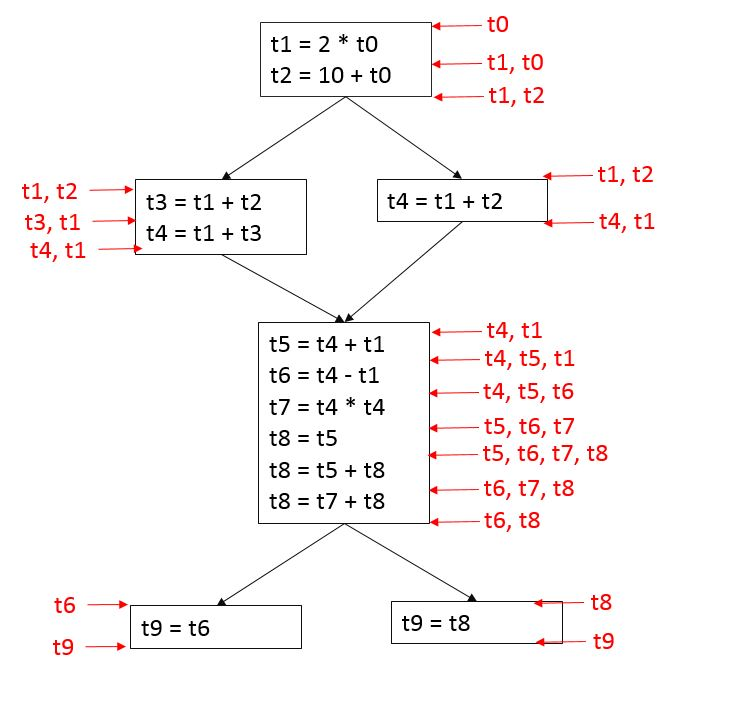
\includegraphics[width=10cm]{1.jpg}
    \end{figure}
    
   \newpage
    \item Provide a lower bound on the number of registers required by the program.\\
    \textbf{Answer:} 
    The lower bound number of registers is 4. 
    
   \newpage
    \item Draw the interference graph between temporaries in the above program as described in class.\\
    \textbf{Answer:} 
       \begin{figure}[h]
    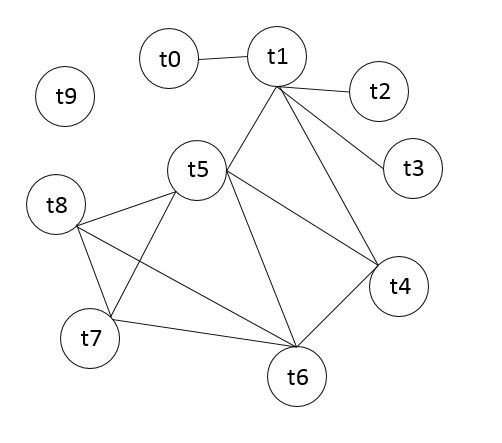
\includegraphics[width=15cm]{2.JPG}
    \end{figure}
    
   \newpage
    \item Using the algorithm described in class, provide a coloring of the above graph. The number of colors used should be your lower bound in part (b). Provide the final k-colored graph (you may use the tikz package to typeset it or simply embed an image), along with the order in which the algorithm colors the nodes.\\
    \textbf{Answer:} 
    stack = {t9, t3, t2, t0, t6, t7, t1, t5, t8, t4} (t9 is the last node into stack, t4 is the first node into stack). 
	The coloring order is from left to right, popping nodes out one by one. 
       \begin{figure}[h]
    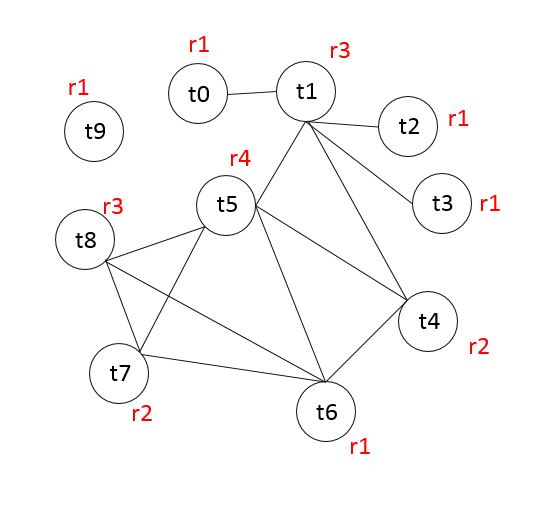
\includegraphics[width=15cm]{3.JPG}
    \end{figure}
    
   \newpage
    \item Based on your coloring, write down a mapping from temporaries to registers (labelled $r1$, $r2$, etc.).\\
    \textbf{Answer:} \\
    {$r1$: $t0$ $t2$ $t3$ $t6$ $t9$}\\
	{$r2$: $t4$ $t7$}\\
	{$r3$: $t1$ $t8$}\\
	{$r1$: $t5$}\\
    
   \newpage
  \end{enumerate}
  
\end{enumerate}
\end{document}